Se realizaron ejecuciones del algoritmo para distintos datasets de grafos de diversos tama'nos y tipo de construcci'on, y se tomaron los tiempos de las mismas.
La siguiente es una tabla con los tama'nos de clique hallado con la Heur'istica Constructiva y tama'no del clique m'aximo .
\footnote{
En http://cs.hbg.psu.edu/benchmarks/clique.html	

SAN (From Laura Sanchis laura@cs.colgate.edu) Instances based on her "Test Case Construction for Vertex Cover Problem," DIMACS Workshop on Computational Support for Discrete Mathematics, March 1992 along with more recent work that will be part of a technical report to be published. The generator generates instances with known clique size.

BROCK (From Mark Brockington brock@cs.ualberta.ca) Instances from Mark Brockington and Joe Culberson's generator that attempts to $"hide"$ cliques in a graph where the expected clique size is much smaller. For more instances, see their generator in graph/contributed/brockington.

PHAT (From Patrick Soriano and Michel Gendreau patrick@crt.umontreal.ca) Random problems generated with the p hat generator which is a generalization of the classical uniform random graph generator. Uses 3 parameters: n, the number of nodes, and a and b, two density parameters verifying 0 $<=$ a $<=$ b $<=$ 1. Generates problem instances having wider node degree spread and larger clique sizes. Reference: "Solving the Maximum Clique Problem Using a Tabu Search Approach", Annals of Operations Research 41, 385-403 (1993).
}

\begin{tabular}{|l|r|r|c|c|r|} 
\hline \multicolumn{6}{|c|}{Data Sets} \\ 
\hline
Parametros & n & m & Cliquemax & Clique hallado & Tiempos[nanoseg] \\ 
\hline \multirow{12}{*}{Brock} 
& 200 & 14834 & 21& 16& 221802186 \\
& 200 & 9876& 12& 8&116371318 \\
& 200& 12048& 15& 9&143049658\\
& 200& 13089& 17& 12& 156085798\\
& 400& 59723& 27& 12& 156251220\\
& 400& 59786& 29& 17& 771334302\\
& 400& 59680& 31& 17& 775103630\\
& 400& 59765& 33& 16& 772941351\\
& 800& 207500& 23& 16& 772895631\\
& 800& 208166& 24& 16& 2667563336\\
& 800& 207333& 25& 16&2684236338\\
& 800& 207646& 26& 13&2463954246\\
\hline \multirow{10}{*}{San} 
& 200 & 13930& 30& 15& 333457562\\
& 200& 13930& 18& 12& 316398773\\
& 200& 17910& 70& 46& 428173815\\
& 200 & 17910& 60& 35& 435356819\\
& 200& 17910& 44& 29& 438124846\\
& 400& 39900& 13& 7& 730263784\\
& 400& 55860& 40& 21& 1391808654\\
& 400& 55860& 30& 15& 1370777747\\
& 400& 55860& 22& 12& 1354123496\\
& 400& 71820& 100& 51& 1824681550 \\
\hline \multirow{10}{*}{PHat} 	
& 300& 10933& -& 4&	230093497 \\
& 300& 21928& -& 12& 597247720 \\
& 300& 33390& -& 26& 816359874  \\
& 500& 31569& -& 5& 584697175 \\
& 500& 62946& -& 13& 1781993497  \\
& 500& 93800& -& 24& 2422429849 \\
& 700& 61000& -& 7& 1513165878 \\
& 700& 121728& -& 17& 3598683796 \\
& 700& 183010& -& 30& 4864516157 \\ 
& 1000& 122253& -& 7& 3053499352 \\
& 1000& 244800& -& 11& 7404595973 \\
& 1000& 371746& -& 31& 10340940720 \\
\hline 
\end{tabular} 

Se observa en la tabla una buena performance del algoritmo, para los grafos de SAN se encontraron cliques de poco mas del 50$%$del tama'no del clique m'aximo, mientras que para los de BROCK que fueron construidos intentando esconder cliques de mayor tama'no en grafos donde se esperan encontrar cliques m'as chicos, la performance es todav'ia un poco mejor. 

 
El siguiente es el gr'afico de los tiempos de corrida en funcion de n*n*log(n), donde podemos comprobar la complejidad calculada anteriormente.
 
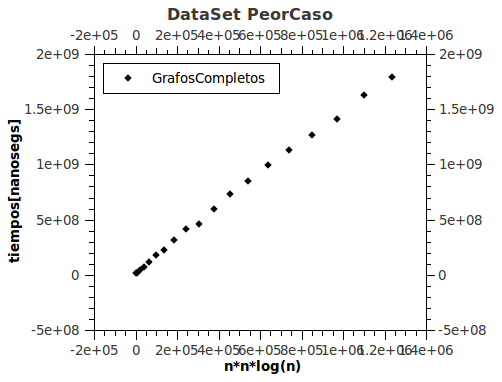
\includegraphics[scale=0.8]{HC/PeorCaso.png}


